%%%%%%%%%%%%%%%%%%%%%%%%%%%%%%%%%%%%%%%%%%%%%%
%% Architectural Decisions
%%%%%%%%%%%%%%%%%%%%%%%%%%%%%%%%%%%%%%%%%%%%%%
\section{Architectural Decisions}
\label{sec:architecture} 

SISDOT is based on the client-server architectural style (according to a typical Java enterprise application), where the components interact to each other by requesting services from other components~\cite{clements2011documenting}. SISDOT is also organized into logical groups of components (known as tiers)---a strategy often used in the client-server architectural style. The multi-tier architectural pattern can be classified as a \emph{component and connector} pattern, depending on the criterion used to define the tiers~\cite{bass2013software}. Indeed, there are several criteria, such as component type, sharing of the execution environment, 
and so on~\cite{clements2011documenting}.

The multi-tier pattern also induces some topological constraints that govern how the components might interact with other components. 
Specifically, connectors might only exist between components of the same tier or that reside in an adjacent tier~\cite{clements2011documenting}. In addition, according to Bass et al., the organization of a system using tiers supports software maintenance, facilitates the definition of security policies, and might increase the performance, availability, and modifiability of 
the systems~\cite{bass2013software}. 



%%%%%%%%%%%%%%%%%%%%%%%%%%%%%%
%% Runtime Architectural Description for QDM Generation
%%%%%%%%%%%%%%%%%%%%%%%%%%%%%%
\subsection{Runtime Architectural Description for QDM Generation}

In order to further detail and illustrate the SISDOT architecture, and the main architectural decisions to address the constraints introduced in Section~\ref{sec:logistics}, here we present a scenario that refers to the generation of QDMs using a runtime architectural description, whose components, relationships, and interactions are illustrated in Figure~\ref{fig:runtime_qdm}). 

\begin{figure}[!ht] %\centering
	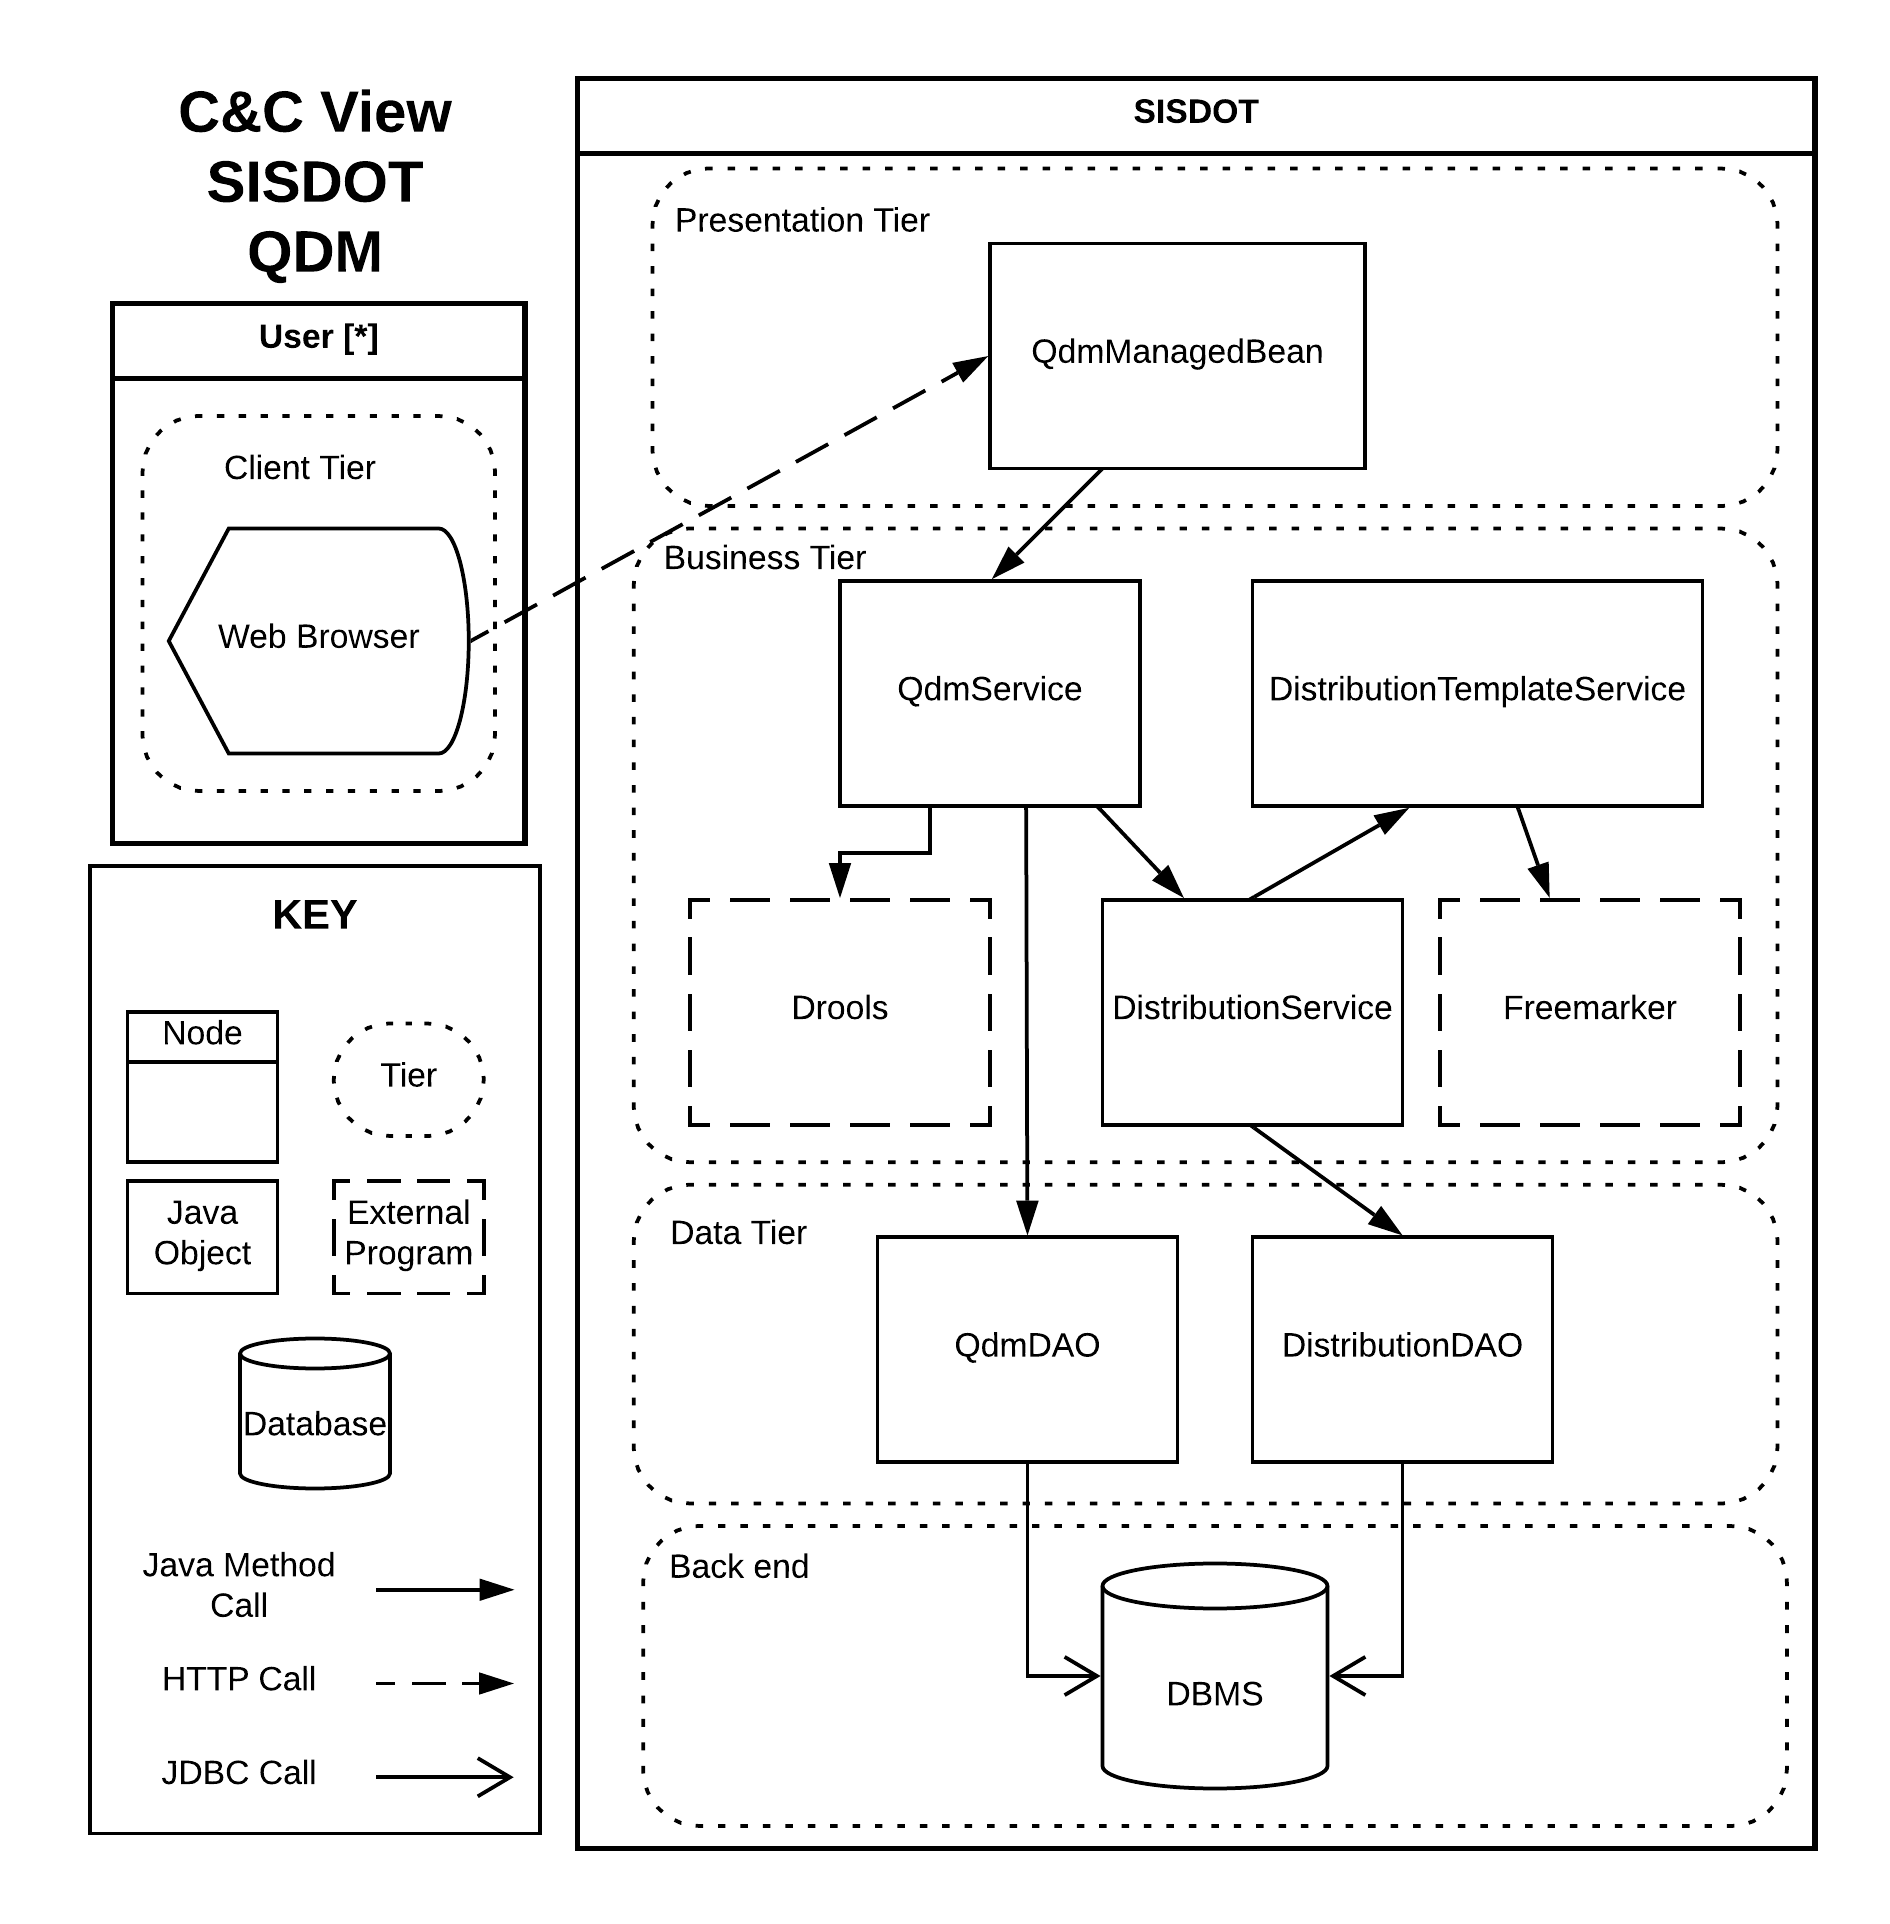
\includegraphics[scale=0.49]{img/runtimeView_qdm.png}
	\caption{Runtime view of the architecture} 
	\label{fig:runtime_qdm}
\end{figure}

\textcolor{red}{arrumar exemplo mais completo de DRL}

\textcolor{red}{falar sobre as regioes da DRL? (qc, fracao, cargo)}

\begin{lstlisting}[frame=single, float=*t, language=DRL, caption=Example of a \emph{low-level Drools rule}, label={code:drl}]
rule "HLR 1"   	
  when
    $qc: QuadroDeCargosVO( 
       (operational == OPERATIONAL || operational == NOT_OPERATIONAL)
       , natureId not in (50, 51)
       , valueId in (23, 41, 90, 50, 42, 31, 21, 32, 20, 30, 40) 
    )	
    $roles: List( size > 0 ) from accumulate ( 
      $dep: DepartmentVO(
         depId not in (14086, 1130)
      ) from $qc.deps 
      and
      $role: RoleVO(
         function == "ROLE"
         , roleId not in (364, 539, 121, 2205, 528, 2204, 539) 
         , rankId in (24, 23, 44, 22, 42) 
         , armsId not in (1055, 10, 833, 5308, 5393, 729, 5110, 15, 5112, 5390, 12) 
      ) from $dep.roles 
      and  		
      QualificationVO(
         code not in ("782", "756", "793", "768", "765", "751", "921", "749", "767", "748")
      ) from $role.qualifications
      and
      ObservationVO(
         code in ("40D","40K")
      ) from $role.observations;
	
      collectList( $role )
    )	 		
  then		 
    for(int i=0; i < $roles.size(); i++){       	
      RoleVO c = (RoleVO) $roles.get(i);
      helper.add(1051000007, c.getDepartmentId(), c.getRoleId());
    }
end
\end{lstlisting}

\emph{Considering the user interaction}, a previously authenticated specialist on the distribution of equipment throughout the Brazilian Army, using her web browser, requests the web page that allows the generation of QDMs (one of the main products of SISDOT). 
After selecting the \emph{generic organizational unity} for which a QDM would be generated, the system sends a request to the server. The client tier is responsible for these actions. The request is then received by a component of the presentation tier, more specifically by a \emph{managed bean} that works as a \emph{front controller} (in this case, a JSF controller). 

This controller validates the request data, before sending a new request to the business tier. In the business tier, the service 
that implements the business rules related to the QDM domain object is invoked to start the QDM generation process, which includes actions to (a) transform \callers into the \emph{low-level rules} specified using the Drools Rule Language (DRL), (b) execute these rules to instantiate a business object that represents a QDM, and (c) save this object in the persistence layer (a relational database). 

This process for generating a QDM starts by retrieving a list of previously registered \callers. An \shc, regardless of its type (either based on the full structure of the organization or based on its components), is related to one or more \emph{military materials / equipment} (MEMs) and defines the respective amount that should be assigned to a military unit (which ranges from an organization, a center, a department, a brigade, or even a military function or qualification of a soldier). 

A high-level rule has one or more distribution rules. Each rule has a type, a value, and an associated description. For example, a rule for a department type has the value of the department identifier and the description of the department name. For a better use of the database, avoiding the definition of numerous columns that would inevitably be null for several rule types, we decided to persist the distribution rules of an \shc using JSON (JavaScript Object Notation), which is converted back to an object when it is retrieved. The set of these rules defines exactly who should receive the MEMs specified by the \shc.

One of the factors that motivated the use of a rule based engine was the similarity between \callers and the ``if-then'' rules of these mechanisms.  %whose essential structure is shown in Listing~\ref{code:drlStructure}.
An \shc has a set of conditions that fits the conditional part of a rule (``if'') and has a set of actions (``then'') that, in this case, trigger the distribution of MEMs throughout the expected military unities.

%\begin{lstlisting}[frame=single, caption={Structure of a rule specified in Drools}, label={code:drlStructure}]
%rule "name"
%    attributes
%    when
%        LHS
%    then
%        RHS
%end
%\end{lstlisting}


The list of retrieved \callers contains only Java objects. In order to be able to use the rule engine in a transparent way for the end users (and also for developers in future maintenance scenarios), we decided to use a meta-programming approach, translating these objects into a set of rules (a program in logic programming) that might be used by a rule-based engine. As mentioned before, we decided to use the \emph{Drools rule-based engine} in the context of SISDOT (Figure \ref{fig:runtime_qdm}), mostly because of its integration capabilities with both JEE systems and the Wildfly application server. Accordingly, the \callers are translated into DRL rules (Listing~\ref{code:drl} presents an example of a \emph{low-level Drools rule}). To this end, we use a template engine (FreeMaker) to implement this particular transformation (Figure \ref{fig:runtime_qdm}), using a template that contains the required \emph{markups} for transforming \shc into \emph{low-level} Drools rules. That is, for each \shc, the template engine populates the template, resulting in a DRL rule consistent with the converted \shc.
% A code snippet of the template used for DRL generation can be seen in Appendix A. 

The RHS of the Drools rule of Listing~\ref{code:drl} iterates over all selected military roles (that satisfy the constraints of the LHS). We use a helper class to assign the equipment id (in this case a \emph{rifle} whose id is 1051000007) to the individual roles. Besides providing means to populate a QDM, this helper class also checks some constraints related to the QDM domain model. 

%\begin{figure}[!ht] \centering
%	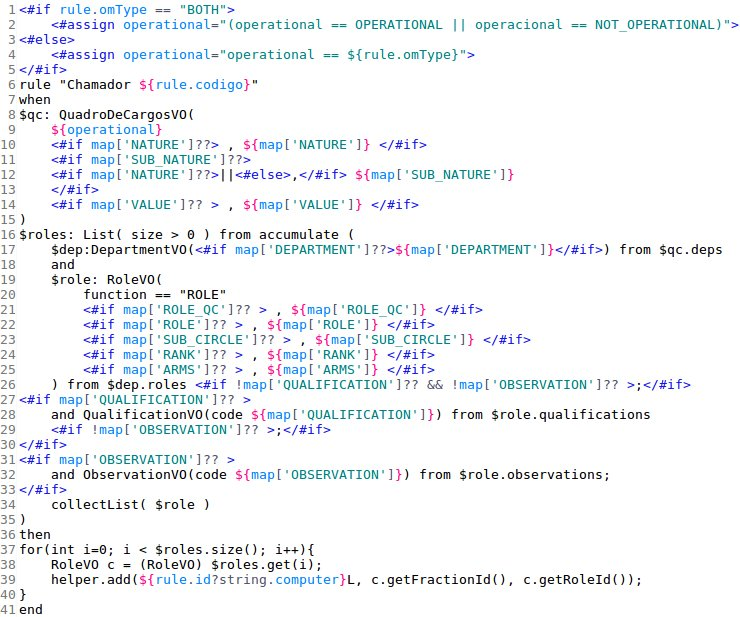
\includegraphics[width=.48\textwidth]{img/artigo_template.jpg}
%	\caption{\it Freemarker template for generating DRL} 
%	\label{fig:template}
%\end{figure}


A QDM is generated for a generic organizational unity (hereafter QC, from \emph{Quadro de Cargos} in Portuguese), selected by the user on the client tier. Therefore, the user-specified QC must be retrieved from the Brazilian Army's enterprise database through a specific Data Access Object (DAO) in the data tier~\cite{alur2003}. From the list of DRL rules, created based on existing \callers, the rule engine is instantiated and these rules are compiled, so that they can be triggered by Drools. The QC domain object is then inserted into the working memory as a fact, an information that is always considered true. The rules are only executed when their conditions are satisfied, based on the specified QC organizational structure. When a rule is valid, that is, it has been activated and the \emph{Left Hand Side} (LHS) conditions are valid, the QDM is populated with the MEMs specified in the \emph{Right Hand Side} (RHS) of the rules. Therefore, we generate a complete QDM object after verifying all valid rules (previously registered in the database) for the selected QC. 

After generating a QDM domain object, it is saved on the database and we let the domain expert know of the success of the operation using a simple user interface message. The domain expert can then perform the necessary operations on the generated QDM, including a workflow involving  its edition, homologation, and validation.  



%%%%%%%%%%%%%%%%%%%%%%%%%%%%%%
%% A Domain Specific Language for testing QDM Generation
%%%%%%%%%%%%%%%%%%%%%%%%%%%%%%
\subsection{A Domain Specific Language for testing QDM Generation}

As explained before, to generate a QDM, a set of \callers must be previously declared. This is a time-consuming task, particularly when using the interface of the system. In order to facilitate the definition of the \callers used in the automated test scripts, we decided to implement \hlrdsl---a DSL (Domain Specific Language) that enables us to specify \callers in a clear, objective, and declarative way (and most important, without using the interface of the SISDOT system). 

We implemented \hlrdsl  using Xtext, which generates plugins that allow code editing in both Eclipse and IntelliJ, plus an editor that can be embedded in a web application. This way, a developer writing test scripts might use \hlrdsl to take advantages of the functionality provided by these plugins. To implement a DSL using Xtext, it is first necessary to declare a grammar expressed using a syntax similar to ANTLR~\cite{parr2013}. Listing~\ref{code:gramatica} presents the grammar of our DSL. From this grammar,the Xtext tool suite generates a lexer, a parser, a set of classes representing the AST (Abstract Syntax Tree), and an editor with several features typically available in IDEs.
% Although Xtext provides an interesting implementation for all these concerns, a language designer is also able to customize several of the Xtext outcomes~\cite{bettini2016}.


\begin{lstlisting}[frame=single, float=*t, language=Xtext, caption={\it Xtext grammar defining the DSL structure}, label={code:gramatica}]
grammar br.unb.cic.sisdot.chamador.HLRDsl 
with org.eclipse.xtext.common.Terminals
generate hlrdsl "http://www.unb.br/sisdot/hlrdsl"

Model:
rules += Rule*;

Rule:
'rule' code = INT '{'
('type' '=' type=OmType ',')?
'materials' '=' '['items+=Item (',' items+=Item)*'],'
'cnds' '=' '['cnds+=Condition (',' cnds+=Condition)*']'
'}';

Item: '(' codot=STRING (':' name=STRING)? ':' amount=INT ')';

Condition:
'(' ('cond' '=' cond=ConditionType ',')?
'type' '=' type = RuleType ','
'values' '=' '[' values+=STRING (',' values+=STRING)* ']'
')';

enum OmType: BOTH | OPERATIONAL | NOT_OPERATIONAL;
enum ConditionType: AFF | NEG;
enum RuleType: NATURE | SUB_NATURE | VALUE | DEPARTMENT | ARMS | ROLE_QC | SUB_CIRCLE | RANK | ROLE | QUALIFICATION | OBSERVATION ;
\end{lstlisting}

Listing \ref{code:dslExample} presents a simple example of a \shc declaration using our DSL. The goal of this rule is to distribute 
the materials (defined in the list of materials construct) for \emph{operational} OMs (see the type construct) and militaries \emph{not working in the specified list of departments} with a set of qualifications and roles. \textcolor{red}{While the definition of this rule using our DSL requires 12 lines of code, the corresponding definition of the same rule using a Java test case requires more than 50 lines of imperative code.}

\begin{small}
	\begin{lstlisting}[frame=single, language=DSL, caption={\it Example of a \shc declaration using our DSL}, label={code:dslExample}]
rule 1 { 
    type = OPERATIONAL, 
    materials = [ 
        ("1051000007" : "Rifle" : 1), 
        ("1020100011" : "Rifle Carrying Case" : 2)
    ], 
    cnds = [ 
        (cond=NEG, type=DEPARTMENT, values=[14086 , 1130]),
        (type=QUALIFICATION, values=[782, 756]), 
        (type=ROLE, values=[2, 12, 15, 21])
    ]
}
	\end{lstlisting}
\end{small}

Our first testing approach consists on the specification of the \callers using \hlrdsl and the specification of the
\emph{behavior under test} using the Cucumber framework~\cite{wynne2017cucumber} (we present an example in Listing \ref{code:cucumber}).
After that, the developer details the implementation steps of the features by (a) specifying which
\callers (previously declared using our DSL) should be considered in the test execution, (b) specifying
which QC the QDM should be generated, and (c) specifying the expected results in terms of the properties
of the expected QDM. To increase productivity, we also implemented a testing  infrastructure that supports several facilities,
including: database connectivity, auxiliary methods for executing queries in the database, and predefined
rules in the rule engine.

{\color{red}That is, \hlrdsl simplifies the process of specifying \callers and its primary goal was to assist in
test activities. However, after presenting to domain experts some examples of \callers specified using our DSL,
we realized that \hlrdsl might also be useful to simulate the specification of rules,
allowing a better understanding of the effect of each \shc for building QDMs.}

\begin{lstlisting}[frame=single, language=Cucumber, caption={\it Cucumber feature}, label={code:cucumber}]
Feature: QDM 757311
As a user
I want to generate a QDM from HLRs

Scenario: Test 1
Given QC with code 757311
And HRL: 1, 2
When I generate a QDM
And the results are consistent
Then positions must be populated
| idDep    | idPos   | codot      | amount |
| 6765748  | 10403   | 1051000025 | 1      |
| 6765748  | 10403   | 1020100017 | 1      |
| 6765748  | 10403   | 1020100013 | 1      |
| 6765748  | 10403   | 1051000006 | 1      |
| 6765748  | 21328   | 1051000025 | 1      |
| 6765750  | 10122   | 1051000025 | 1      |    
| 6765793  | 13276   | 1051000025 | 6      |
| 6765796  | 24655   | 1051000025 | 1      |
| 6765796  | 24429   | 1051000025 | 2      |
| 6765798  | 24429   | 1051000025 | 3      |
| 6765798  | 11433   | 1051000025 | 9      |   
And the final result must be:
| codot      | amount |
| 1020100013 | 74     |
| 1020100017 | 74     |
| 1051000006 | 74     |
| 1051000025 | 74     |

\end{lstlisting}

Our second testing approach automatically generates test cases from our DSL and from a random sample of simple combinations that simulate organizational unities. This \emph{property based approach} involves a custom Maven plugin that currently generates random scenarios, freeing the tester to only implement more complex tests related to the QDM generation. 

\textcolor{red}{These test cases are generated from a combination of conditions, for example: one test case only for operational OMs and another for non-operational OMs; a test case for the different kinds of OMs (artillery, infantry, cavalry, aviation and helicopters, general services, and so on), combining with the operational type, such as: operational infantry OMs and non-operational infantry OMs. These combinations are generated for simple cases so that they are easy to verify without the need to manually implement Java test scripts for generating QDMs.}

% O Maven plugin desenvolvido define diversos cenários que serão gerados para cada QC declarado. Cada cenário é responsável pela geração de uma high-level rules no formato DSL e um arquivo de definição do cenário no formato do cucumber. Para cada cenário é gerado um QDM para o QC, usando a high-level rule gerado e o resultado deste QDM é conferido de acordo com os dados previstos na definição do cenário do cucumber. Foram criadas diversas combinações de cenários e para cada uma delas alguns dos valores das propriedades são gerados randomicamente, seguindo a técnica PBT. 

The Maven plugin developed defines several scenarios that will be generated for each declared QC. Each scenario is responsible for generating high-level rules using\hlrdsl and a scenario definition file using Cucumber features. For each scenario, a QDM for the QC is generated, using the generated high-level rule and the result of this QDM is checked according to the predicted data in the Cucumber scenario definition. Several combinations of scenarios have been created and for each of them some of the values of the properties are generated randomly, following the PBT technique.

% Os cenários de teste foram divididos em três grupos, de acordo com as seções da DRL (QC, fração e cargo). Isso foi feito pois cada região é testada de forma quase que independente, possuindo dependência apenas da validade da região anterior. Por exemplo: a região de fração só é avaliada se a região de QC tiver sido avaliada como verdadeira, então essas regiões podem ser testadas de forma independente ao assumir que a região anterior é verdadeira e que foram gerados casos de testes que ajudaram a validar o funcionamento das condições da região anterior. Ao assumir a independência dos grupos, para fins de teste, é possível focar nas combinações das propriedades de cada grupo, facilitando a geração de cenários de teste. 

The test scenarios were divided into three groups, according to the sections of the DRL (QC, fraction and charge). This was done because each region is tested almost independently, having dependence only on the validity of the anterior region. For example: the fraction region is evaluated only if the QC region has been evaluated as true, then these regions can be tested independently by assuming that the previous region is true and that test cases have been generated which have helped to validate the conditions of the previous region. By assuming the independence of the groups, for testing purposes, it is possible to focus on the combinations of the properties of each group, facilitating the generation of test scenarios.

% Cada grupo de cenários é responsável por testar várias das combinações das propriedades da entidade relativa ao grupo (QC, fração ou cargo). Em cada cenário é definido uma high-level rule e uma lista com os resultados esperados, que são gerados de acordo com a combinação específica de propriedades deste cenário. Como o MEM definido na high-level rule não interfere na execução das regras, foi definido um MEM padrão para todas as high-level rules geradas, assim como a quantidade igual a um (unitário). Isso foi feito para diminuir a complexidade do algoritmo de geração ao não precisar acessar o banco de dados várias vezes para recuperar MEMs de forma randômica, tendo em vista que não interferem na avaliação das regras envolvidas na geração do QDM.

Each scenario group is responsible for testing different combinations of entity properties relative to the group (QC, fraction or charge). In each scenario a high-level rule and a list with the expected results are defined, which are generated according to the specific combination of properties in this scenario. Since the MEM defined in the high-level rule does not interfere in the execution of the rules, a standard MEM has been defined for all high-level rules generated, as well as a quantity equal to one (unitary). This was done to reduce the complexity of the generation algorithm by not having to access the database several times to retrieve MEMs in a random way, since they do not interfere in the evaluation of the rules involved in the generation of QDM.

% No grupo de QC existem as seguintes propriedades: operacionalidade, natureza, subnatureza e valor. Foram criados cenários específicos para cada propriedade e para combinações entre elas. Para a propriedade natureza do QC, por exemplo, foram definidos os seguintes cenários:

There are four domain properties related to QCs:
\emph{kind} (either operational, non-operational or both),
\emph{nature}, \emph{sub-nature}, and \emph{value}. Specific scenarios have been created not only for each property, but also considering different
combinations of properties. For instance, considering the \emph{nature} property of the QC,
the following scenarios have been defined:

\begin{itemize}

% \item natureza válida e tipoOM válido: este cenário gera um QDM válido, com resultados válidos, pois neste cenário é criado um high-level rule com os mesmos valores de natureza e operacionalidade (tipoOM) do QC para o qual será gerado o QDM, ou seja, natureza e tipoOM válidos;

\item valid nature and valid OM type: this scenario generates a valid QDM, with valid results, because in this scenario a high-level rule with the same values of nature and type of the QC for which the QDM is generated is created , valid nature and typeOM;

% \item natureza válida e tipoOM válido (AMBOS): este cenário funciona de forma parecida com o anterior, mas o tipoOM é definido como "AMBOS" no high-level rule. Este tipoOM indica que o QC pode ser operacional ou não-operacional;

\item valid type and valid typeOM (BOTH): this scenario works similarly to the previous one, but the typeOM is set to "BOTH" in the high-level rule. This type indicates that QC can be operational or non-operational;

% \item natureza válida e tipoOM inválido: o valor da natureza é o mesmo do QC, pois é válido, e o valor do tipoOM é alterado. Por exemplo: se o QC for operacional o valor é alterado para não-operacional e vice-versa;

\item valid nature and invalid typeOM: the value of nature is the same as the QC, since it is valid, and the value of typeOM is changed. For example: if the QC is operational the value is changed to non-operational and vice versa;

% \item natureza inválida e tipoOM válido: o valor da natureza deve ser inválido no high-level rule, ou seja, um valor diferente da natureza do QC. A geração deste valor inválido de natureza é realizado de forma randômica, usando a seed configurada no plugin maven, em uma lista de códigos de naturezas reais previamente definida;

\item Invalid nature and valid typeOM: Nature value must be invalid at high-level rule, i.e., a value different from the nature of QC. The generation of this invalid value of nature is performed in a random fashion, using the seed configured in the maven plugin, in a previously defined real-life code list;

% \item natureza inválida e tipoOM inválido: os valores de natureza e tipoOM são inválidos, e são gerados conforme citado anteriormente: invertendo o valor de operacionalidade e recuperando randomicamente um código de natureza da lista declarada previamente;

\item Invalid nature and invalid typeOM: the values of nature and typeOM are invalid, and are generated as previously mentioned: reversing the value of operability and randomly retrieving a code of nature from the list previously declared;

% \item negar natureza, inválido: as combinações citadas anteriormente nesta lista possuem high-level rules com regras do tipo "AFIRMACAO", o tipo padrão de uma regra. Mas existe o tipo "NEGACAO", onde a regra é negada, ou seja, a condição (na DRL) é válida quando o valor testado não pertence à lista de valores especificados na regra. Neste cenário, por exemplo, há uma regra de negação da natureza de forma que o QDM seja inválido. Então foi criada uma regra para "NATUREZA" do tipo "NEGACAO" definindo como valor o código da natureza do QC. Com isso, esta regra não é válida para este QC, sendo válida para todas as outras naturezas exceto a deste QC;

\item deny nature, invalid: the combinations previously mentioned in this list have high-level rules with rules of type "AFFIRMATION", the standard type of a rule. But there is the type "DENIAL", where the rule is denied, that is, the condition (in the DRL) is valid when the value tested does not belong to the list of values specified in the rule. In this scenario, for example, there is a nature negation rule so that QDM is invalid. Then a rule for "NATURE" of the type "DENIAL" was created defining the code of the nature of QC. Therefore, this rule is not valid for this QC, being valid for all other natures except that of this QC;

% \item negar natureza, válido: para este cenário é criado uma high-level rule com uma regra para "NATUREZA" do tipo "NEGACAO", mas gerando um código de natureza diferente da natureza do QC. Com isso, esta regra é válida para este QC.

\item deny nature, valid: for this scenario a high-level rule with a rule for "NATURE" of type "DENIAL" is created, but generating a code of a nature different from the nature of QC. Therefore, this rule is valid for this QC.
\end{itemize}

% Seguindo a mesma linha de combinações utilizadas paras cenários envolvendo natureza do QC, foram criados cenários para subnatureza e valor. Não foram criados cenários para tipoOM pois esta é uma propriedade de preenchimento obrigatório no high-level rule e a checagem de sua validade já é exercitada em todos os cenários do grupo. Na Table \ref{table:valor} são apresentados os cenários definidos para o Valor do QC e suas combinações. Na primeira coluna é apresentado o número do cenário, criado apenas para facilitar uma possível referência a uma linha específica da tabela. As outras colunas contém os valores das propriedades do QC sendo combinadas. A células com valor 0 indicam que o valor desta propriedade, indicada pela coluna, é inválido, ou seja, deverá ser selecionado um valor randomicamente de uma lista previamente definida e este valor deve ser diferente do valor que essa propriedade apresenta no QC. As células com o valor 1 indicam que o valor desta propriedade é válido, ou seja, é o mesmo valor definido no QC para esta propriedade. As células sem valor indicam que essa propriedade não faz parte da combinação. 

Following the same line of combinations used for scenarios involving the nature of QC, scenarios were created for sub-nature and value. No scenarios have been created for typeOM because this is a mandatory property in the high-level rule and checking its validity is already exercised in all scenarios of the group. In Table \ref{table:valor} the scenarios defined for the Value of QC and its combinations are presented. In the first column the scenario number is displayed, created only to facilitate a possible reference to a specific row in the table. The other columns contain the QC property values being combined. Cells with a value of 0 indicate that the value of this property, indicated by the column, is invalid, that is, a random value must be selected from a previously defined list and this value must be different from the value that this property has in QC. Cells with a value of 1 indicate that the value of this property is valid, that is, it is the same value defined in the QC for this property. Cells with no value indicate that this property is not part of the combination.

\begin{table}[htb!]
	\centering
	\caption{Defined Scenarios for QC Value}
	\label{table:valor}
	\begin{center}
		\begin{tabular}{ccccc}
			\toprule
\textbf{Scenarios} & \textbf{Value} & \textbf{Subnature} & \textbf{Nature} & \textbf{TypeOM} \\ \hline
1                & 0              &                      &                   & 0               \\ \hline
2                & 0              &                      &                   & 1               \\ \hline
3                & 1              &                      &                   & 0               \\ \hline
4                & 1              &                      &                   & 1               \\ \hline
5                & 0              &                      & 0                 & 0               \\ \hline
6                & 0              &                      & 0                 & 1               \\ \hline
7                & 0              &                      & 1                 & 0               \\ \hline
8                & 0              &                      & 1                 & 1               \\ \hline
9                & 1              &                      & 0                 & 0               \\ \hline
10               & 1              &                      & 0                 & 1               \\ \hline
11               & 1              &                      & 1                 & 0               \\ \hline
12               & 1              &                      & 1                 & 1               \\ \hline
13               & 0              & 0                    & 0                 & 0               \\ \hline
14               & 0              & 0                    & 0                 & 1               \\ \hline
15               & 0              & 0                    & 1                 & 0               \\ \hline
16               & 0              & 0                    & 1                 & 1               \\ \hline
17               & 0              & 1                    & 0                 & 0               \\ \hline
18               & 0              & 1                    & 0                 & 1               \\ \hline
19               & 0              & 1                    & 1                 & 0               \\ \hline
20               & 0              & 1                    & 1                 & 1               \\ \hline
21               & 1              & 0                    & 0                 & 0               \\ \hline
22               & 1              & 0                    & 0                 & 1               \\ \hline
23               & 1              & 0                    & 1                 & 0               \\ \hline
24               & 1              & 0                    & 1                 & 1               \\ \hline
25               & 1              & 1                    & 0                 & 0               \\ \hline
26               & 1              & 1                    & 0                 & 1               \\ \hline
27               & 1              & 1                    & 1                 & 0               \\ \hline
28               & 1              & 1                    & 1                 & 1               \\ \hline
		\end{tabular}
	\end{center}
\end{table}

% No grupo Cargo existem as seguintes propriedades: código do cargo, subcírculo ao qual o cargo pertence, o posto (patente) necessário para ocupar o cargo, e a arma (Arma, Quadro ou Serviço) necessária para ocupar o cargo. O subcírculo está relacionado às graduações (posto/patente) existentes, servindo como uma forma de agrupamento. Por exemplo: o subcírculo superior agrupa as patentes de coronel, tenente-coronel e major; o subcírculo subalterno agrupa os tenentes. 

In the Cargo group there are the following properties: position code, sub-circle to which the position belongs, position (patent) needed to fill the position, and the weapon (Weapon, Frame or Service) required to fill the position. The sub-circle is related to existing (rank/patent) grades, serving as a form of grouping. For example: the upper sub-circle groups the patents of colonel, lieutenant-colonel and major; the subordinate sub-circle groups the lieutenants.

% Para cada cenário do grupo de cargos foi selecionado um cargo aleatoriamente da lista de cargos do QC, utilizando a seed configurada no plugin maven. De acordo com o cargo selecionado são geradas as regras conforme a combinação de propriedades especificada para o cenário. Para cada cenário, além das regras, é gerada também uma lista contendo os resultados esperados, ou seja, os dados que se espera encontrar no QDM gerado para o QC. 

For each scenario in the job group, a job was randomly selected from the QC job list, using the seed configured in the maven plugin. According to the selected position, the rules are generated according to the combination of properties specified for the scenario. For each scenario, in addition to the rules, a list containing the expected results is generated, that is, the data expected to be found in the QDM generated for the QC.

% Para este trabalho foram especificados 100 cenários. Todos os cenários gerados, independente do grupo, contém um high-level rule, com as regras referentes à combinação de propriedades definida para o cenário, e uma lista de resultados esperados, que serão comparados com os dados do QDM gerado. Para cada QC declarado no plugin é gerada uma lista de cenários. Para cada QC é gerado um arquivo cucumber contendo os cenários definido para este QC. A geração do arquivo é realizada com o uso do Freemarker, usando um template previamente definido.

For this work 100 scenarios were specified. All generated scenarios, independent of the group, contain a high-level rule, with rules relating to the combination of properties defined for the scenario, and a list of expected results that will be compared with the generated QDM data. For each QC declared in the plugin a list of scenarios is generated. For each QC is generated a cucumber file containing the scenarios defined for this QC. File generation is done using Freemarker, using a predefined template.

% O processo de geração automática de testes pode ser resumido da seguinte maneira: o plugin maven deve ser declarado e configurado, indicando a lista com os códigos dos QCs para os quais devem ser gerados testes. Então, para cada QC da lista são gerados cenários, com variações em suas propriedades de acordo com o QC sendo testado. Os cenários gerados são transformados em arquivos do cucumber e de DSL, que representam os cenários gerados. Houve então uma conversão dos cenários gerados com base na técnica Property-based Testing (PBT) em casos de teste, por exemplo, que serão executados automaticamente durante a fase adequada do ciclo de vida de \textit{build} do maven. Existe a possibilidade de geração de relatório da execução dos testes em alguns formatos, como: html e json.

The automatic test generation process can be summarized as follows: The maven plugin must be declared and configured, indicating the list of QC codes for which tests must be generated. Then, for each QC of the list scenarios are generated, with variations in their properties according to the QC being tested. The generated scenarios are transformed into cucumber and DSL files, which represent the generated scenarios. There was then a conversion of the generated scenarios based on the Property-based Testing (PBT) technique into test cases, for example, that will run automatically during the appropriate maven build phase. There is the possibility of reporting the execution of tests in some formats, such as: html and json.

% \begin{lstlisting}[frame=single, language=Plugin, caption={\it Maven plugin for test generation}, label={code:plugin}]
% <plugin>
%   <groupId>xxx</groupId>
%   <artifactId>xxx</artifactId>
%   <executions>
%     <execution>
%       <id>execute</id>			
%       <configuration>
%         <seed>10</seed>				
%         <qcs>702311,762314,575311</qcs>				
%       </configuration>
%       <goals>
%         <goal>generate</goal>
%       </goals>
%     </execution>
%   </executions>
% </plugin>	
% \end{lstlisting}

\textcolor{red}{In this second approach, for each of the possible combinations, we generate a \shc that meets the conditions and a cucumber feature that exercises the \shc and compares the expected results declared in the feature. Each \shc is considered during the generation of the QDM to the QCs specified in the maven plugin.
That is, to use this architecture characteristic (here we consider testability as an architecture concern), we ``feed'' the maven plugin with a list of QC codes for which the QDMs should be generated, besides other optional information, which have default values, such as: database connection string, seed to be used in the random selection of values within a combination (e.g., considering 20 different kinds of organizational unities, randomly take 5 for generating the set of combinations), and the output directory where the code should be exported. }

After running the plugin, with the generated code, the tests are executed in a similar way to the test definitions detailed before. The tests run along with the other unit tests declared, whether DSL-based or not.

